% Created 2022-02-22 mar 18:39
% Intended LaTeX compiler: pdflatex
\documentclass[conference]{IEEEtran}
\usepackage[utf8]{inputenc}
\usepackage[T1]{fontenc}
\usepackage{graphicx}
\usepackage{longtable}
\usepackage{wrapfig}
\usepackage{rotating}
\usepackage[normalem]{ulem}
\usepackage{amsmath}
\usepackage{amssymb}
\usepackage{capt-of}
\usepackage{hyperref}
\input{~/org/latex/author_TecDig2_Riedinger-Garcia.tex}
\input{~/org/latex/ieee.tex}
\date{\today}
\title{Sistema de adquisión y transmisión de datos autosuficiente y controlable - Manual de Servicio}
\hypersetup{
 pdfauthor={},
 pdftitle={Sistema de adquisión y transmisión de datos autosuficiente y controlable - Manual de Servicio},
 pdfkeywords={},
 pdfsubject={},
 pdfcreator={Emacs 27.2 (Org mode 9.6)}, 
 pdflang={Spanish}}
\begin{document}

\maketitle
\tableofcontents


\section{Consideraciones de seguridad:}
\label{sec:org6dcd27d}
\subsection{Riesgos y procedimientos de seguridad:}
\label{sec:org69151f7}
Ambos sistemas operan niveles de bajos de voltaje, por lo que los riesgos al realizar los mantenimientos son mínimos. Sin embargo, se deben tener las siguientes precauciones al operar:

\begin{itemize}
\item Utilizar calzado y pulseras antiestáticas para evitar el daño a los equipos.
\item Desconectar de la alimentación ambos sistemas antes de realizar el mantenimiento (aunque sea de solo un sistema en particular).
\item Desconectar la conexión USART entre ambos sistemas antes de realizar el mantenimiento de uno de los mismos.
\end{itemize}
\section{Herramientas y equipos para realizar el servicio:}
\label{sec:org797bdca}
\subsection{Herramientas e instrumental necesario:}
\label{sec:org86daaff}
Será necesario para realizar el mantenimiento las siguientes herramientas:

\begin{itemize}
\item Destornilladores tipo paleta y Philips para realizar el desamblaje de las carcasas de los equipos.
\item Multímetro digital o analógico para corroborar los valores de referencia (con el sistema encendido para realizar mediciones de voltaje y con el sistema desconectado para realizar mediciones de continuidad).
\item Osciloscopio digital u analógico para corroborar las señales de referencia (con el sistema conectado).
\item Manuales de usuario de los elementos anteriores y de los siguientes:
\begin{itemize}
\item STM32F429ZI-Nucleo.
\item LM35Z.
\item LM358.
\end{itemize}
\end{itemize}
\subsection{Software y aplicaciones necesarias:}
\label{sec:org5835b3d}
Para comprobar y debugger el código embebido en el sistema será necesario el programa libre de ST Atollic TRUEStudio. Indiferentemente, también es posible utilizar cualquiera de las opciones ofrecidas por ST o algún otro programa basado en Eclipse, pero se aclara que el programa de ambos sistemas fue debuggeado en Atollic TRUEStudio y solo probado en el mismo.

Luego, para editar los archivos del PCB será necesario el software Proteus 8.12 SP0 Professional.

Todos los archivos de software se pueden encontrar en la página oficial de GitHub del proyecto: \url{https://github.com/AugustoRiedinger/tecDig2\_project}.
\section{Diagramas de circuito}
\label{sec:orgffac52a}
\subsection{Diagrama general en bloques:}
\label{sec:org06a1864}
\begin{figure}[htbp]
\centering
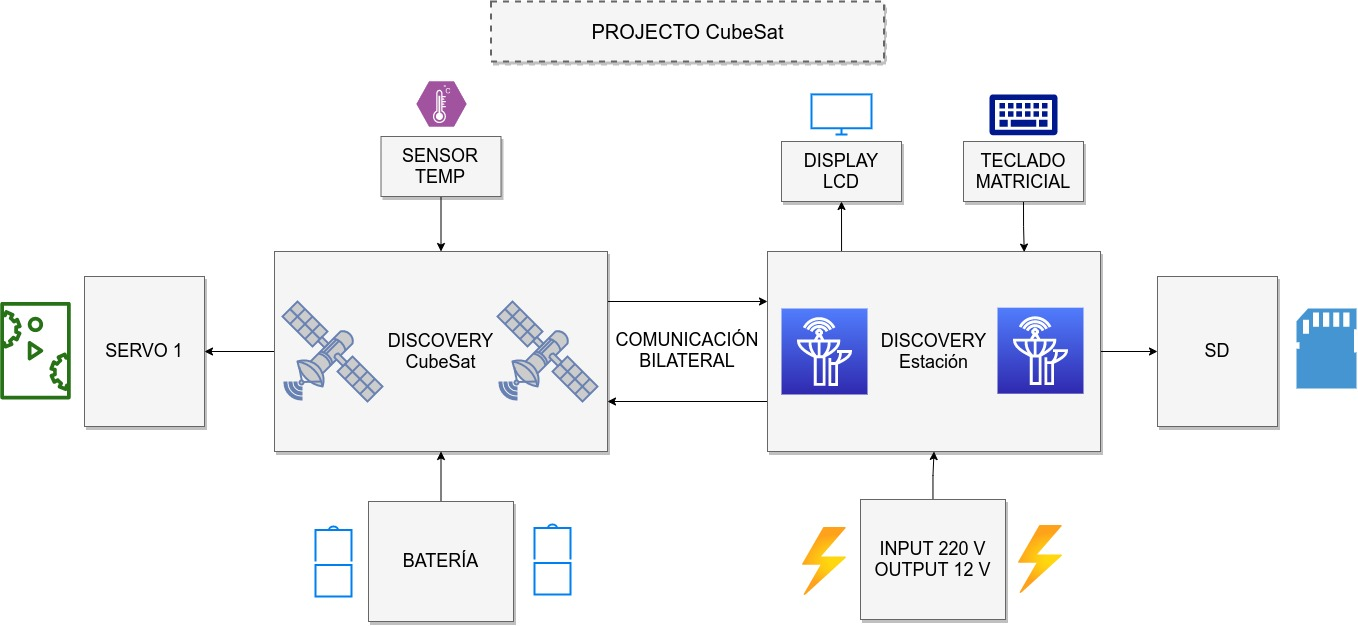
\includegraphics[width=.9\linewidth]{../../images/diagramaBloques.jpg}
\caption{\label{fig:diagramaBloques}Diagrama general en bloques}
\end{figure}

En la Fig. \ref{fig:diagramaBloques} se puede observar el diagrama en bloques general del sistema. El mismo describe gráficamente cada una de las funcionalidades y aplicaciones del sistema.
\subsection{Circuitos esquemáticos y PCB:}
\label{sec:org43b238f}
En la Fig. \ref{fig:estacionEsquematico} se puede visualizar el esquemático de la ERDYTC para realizar el mantenimiento.

\begin{figure}[htbp]
\centering
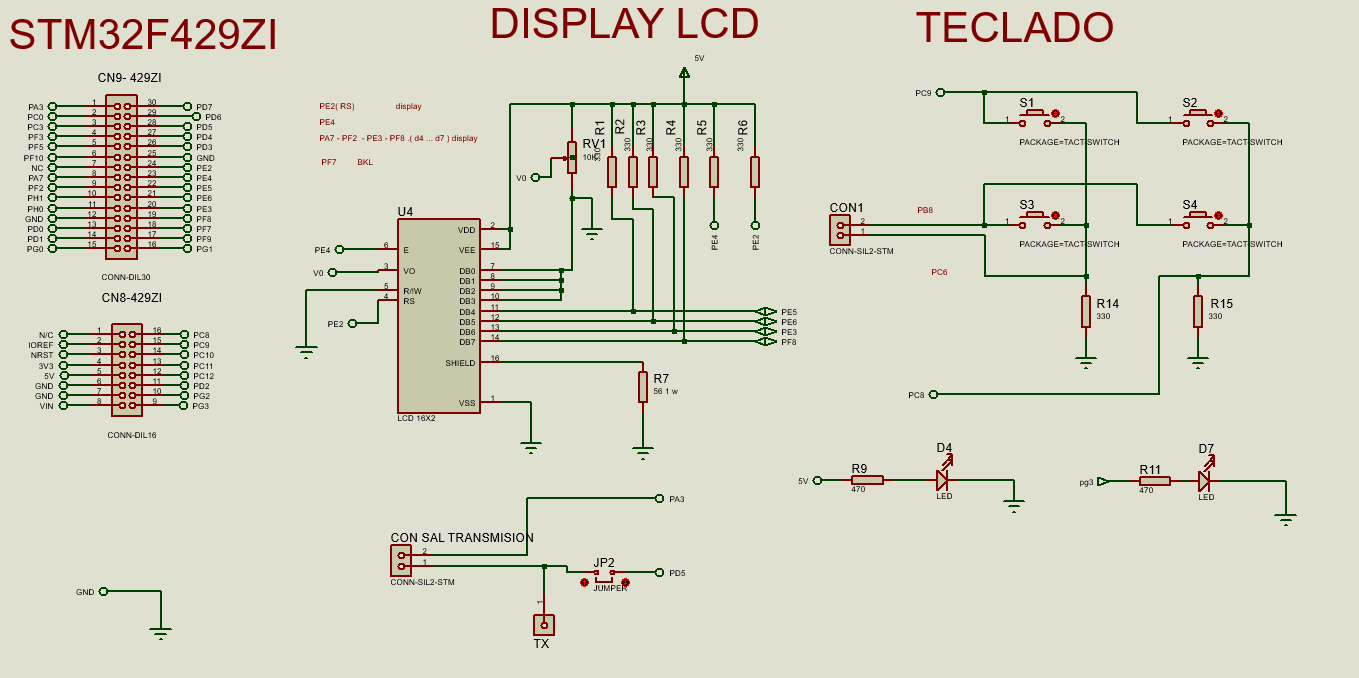
\includegraphics[width=.9\linewidth]{../../images/estacionEsquematico.png}
\caption{\label{fig:estacionEsquematico}Esquemático ERDYTC}
\end{figure}

En la Fig. \ref{fig:cuboEsquematico} se puede visualizar el esquemático del SATDAC para realizar el mantenimiento.

\begin{figure}[htbp]
\centering
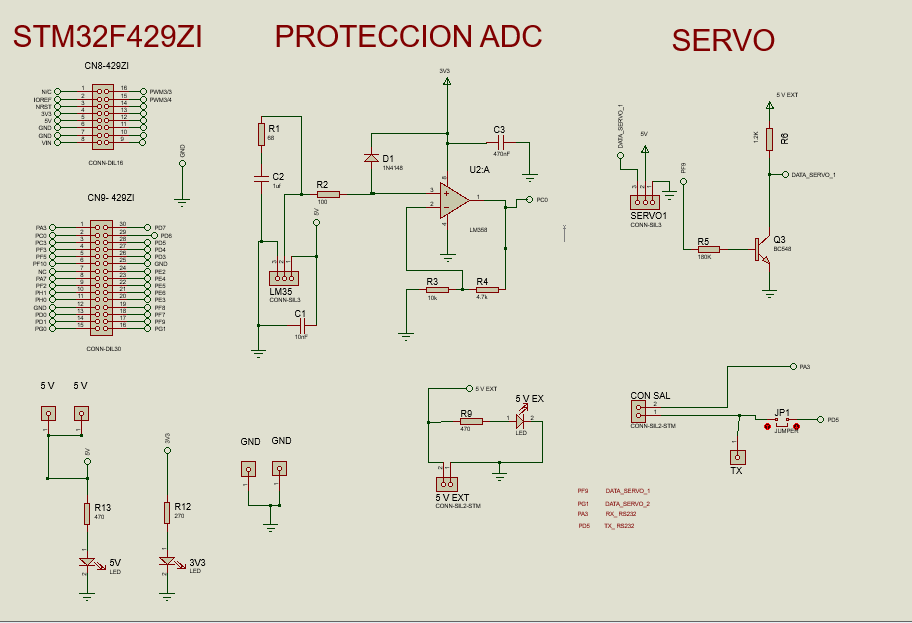
\includegraphics[width=.9\linewidth]{../../images/cuboEsquematico.png}
\caption{\label{fig:cuboEsquematico}Esquemático SATDAC}
\end{figure}

\subsection{Descripción de conectores y jumpers:}
\label{sec:org6677738}
Los conectores principales utilizados en el sistema son de alimentación:

\begin{itemize}
\item En la ERDYTC, el conector de alimentación se puede desamblar a partir del transformador que se conecta a la red, no es necesario realizar la desconexión de la STM.
\item En el SATDAC, el conector de alimentación es recomendable sacarlo directamente de la STM.
\end{itemize}

Luego, ambos sistemas cuentan en sus respectivas PCB con LEDs de estado para indicar que el sistema está alimentado.

Finalmente, ambos PCB también cuentan con un JUMPER J1 para cambiar el pin de conexión del TX de ambos sistemas. Este pin debe ser dejado abierto a menos que se cambie desde el software la conexión del TX-USART en los respectivos sistemas.
\section{Mediciones y ajustes:}
\label{sec:orgd5a399b}
\subsection{Puntos de referencia:}
\label{sec:org0bfd5c2}
Ambos sistemas cuentan con LEDs marcados testigos que indican los diferentes bloques de tensión. En el mantenimiento, se debería verificar primeramente que todos los LEDs de los PCB se encuentren encendidos. De no ser así, se puede rastrear a partir de los mismos y del los esquemáticos el punto de error.
\subsection{Señales de referencia:}
\label{sec:orga26c996}
La única señal de referencia que poseen ambos sistemas es la del servomotor en el SATDAC.

La misma emana del puerto PG0, o hacia la base del transitor amplificador corte-saturación T1. Se debería verificar que dicha señal sea un pulso cuadrado de período 50 [Hz] con un ancho en cero de 1 milisegundo.

Alternativamente, se puede verificar la señal inversa en el colector del transistor T1, como un pulso de también 50 [Hz] y un ancho en "1" de 1 milisegundo.

El ajuste de estas ondas debe ser realizado exclusivamente por software.
\section{Procedimientos de reemplazo:}
\label{sec:org224fde4}
\subsection{Módulos:}
\label{sec:orgf8061fa}
Ambos sistemas cuentan con PCB realizados en poncho; por tanto, en caso de que los microcontroladores no funcionen, los mismos se pueden reemplazar fácilmente al desamblar la PCB del módulo.
\section{Mensajes de error:}
\label{sec:orgcc5377a}
El único mensaje de error que poseen los sistemas se da en el ERDYTC; y se puede visualizar en la Fig. \ref{fig:error}.

\begin{figure}[htbp]
\centering
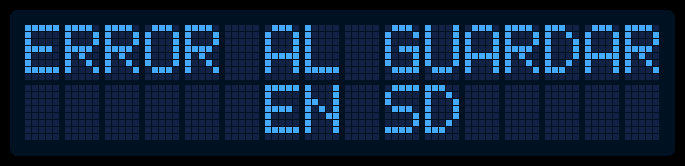
\includegraphics[width=.9\linewidth]{../../images/error.png}
\caption{\label{fig:error}Menaje de error SD}
\end{figure}

El mismo indica que no se pudieron guardar datos en la SD. En caso de ver este error, es recomendable verificar primeramente el módulo SD se encuentre bien conectado en el SATDAC.

Para ello, primero se debe pulsar el pulsador 2 para abrir la compuerta del SATDAC; y luego de desconectar el conexionado entre ambos sistemas y sus alimentaciones, verificar la correcta conexión del módulo SD como se indica en el esquemático.

Luego, se debe cerrar manualmente la compuerta con el servomotor y a partir de allí volver a realizar todas las conexiones. Si aún así se visualiza este mensaje luego de presionar el pulsador 3; es recomendable realizar el procedimiento anterior y cambiar el módulo SD.
\section{Lista de partes y reemplazos:}
\label{sec:org100c06f}
En las Fig. \ref{fig:estacionBOM} y \ref{fig:cuboBOM} se pueden visualizar los componentes que componen cada sistema respectivamente.

\begin{figure}[htbp]
\centering
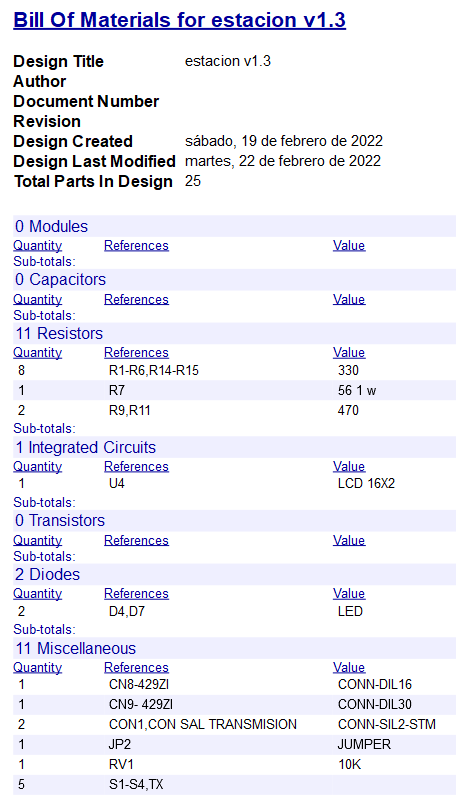
\includegraphics[width=.9\linewidth]{../../images/estacionBOM.png}
\caption{\label{fig:estacionBOM}ERDYTC partes}
\end{figure}

\begin{figure}[htbp]
\centering
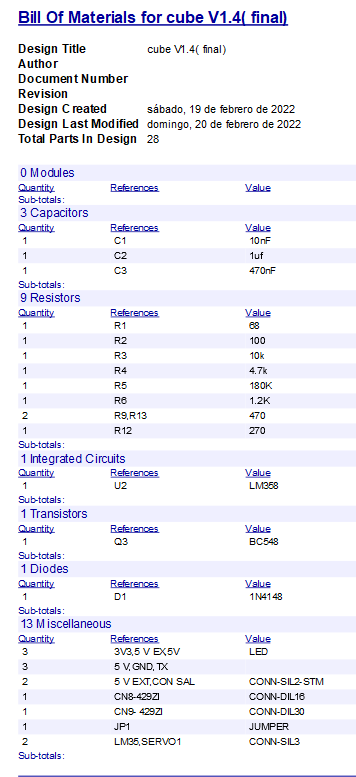
\includegraphics[width=.9\linewidth]{../../images/cuboBOM.png}
\caption{\label{fig:cuboBOM}SATDACT partes}
\end{figure}

Es aconsajable que, en caso de reemplazo, se cambien los componetes por los listados anteriormente. De no ser así, se aconseja buscar los modelos más parecidos.
\section{Información y soporte:}
\label{sec:orgb8b5b1a}
Cualquier pregunta es aconsajable el contacto hacia los autores o en el siguiente enlace: \url{https://www.openstm32.org/forums}.
\end{document}
